\documentclass[notitlepage,11pt]{article}
\usepackage[margin=0.8in]{geometry}
\usepackage{enumitem}
\usepackage{textcomp}
\usepackage{amsmath}
\usepackage{graphicx}
\usepackage{listings}
\usepackage{color}
\usepackage{float}
\usepackage{hyperref}
\usepackage{array}

\definecolor{codegreen}{rgb}{0,0.6,0}
\definecolor{codegray}{rgb}{0.5,0.5,0.5}
\definecolor{codepurple}{rgb}{0.58,0,0.82}
\definecolor{backcolour}{rgb}{0.95,0.95,0.92}
 
\lstdefinestyle{mystyle}{
    backgroundcolor=\color{backcolour},   
    commentstyle=\color{codegreen},
    keywordstyle=\color{magenta},
    numberstyle=\tiny\color{codegray},
    stringstyle=\color{codepurple},
    basicstyle=\footnotesize,
    breakatwhitespace=false,         
    breaklines=true,                 
    captionpos=b,                    
    keepspaces=true,                 
    numbers=left,                    
    numbersep=5pt,                  
    showspaces=false,                
    showstringspaces=false,
    showtabs=false,                  
    tabsize=2
}

\newcolumntype{C}[1]{>{\centering\arraybackslash}p{#1}} % new col type that allows for wrapped text
 
\lstset{style=mystyle}

\linespread{1.5}
\setlength{\parindent}{1cm} % Default is 15pt.

\title{\textbf{Automated Pet Feeder} \\ Final Report Proposal}
\author{Robinson Merillat \and Victoria Bennett}
\date{May 7, 2018}

\begin{document}
    \maketitle
    \begin{center}             % centers whateve is inside
        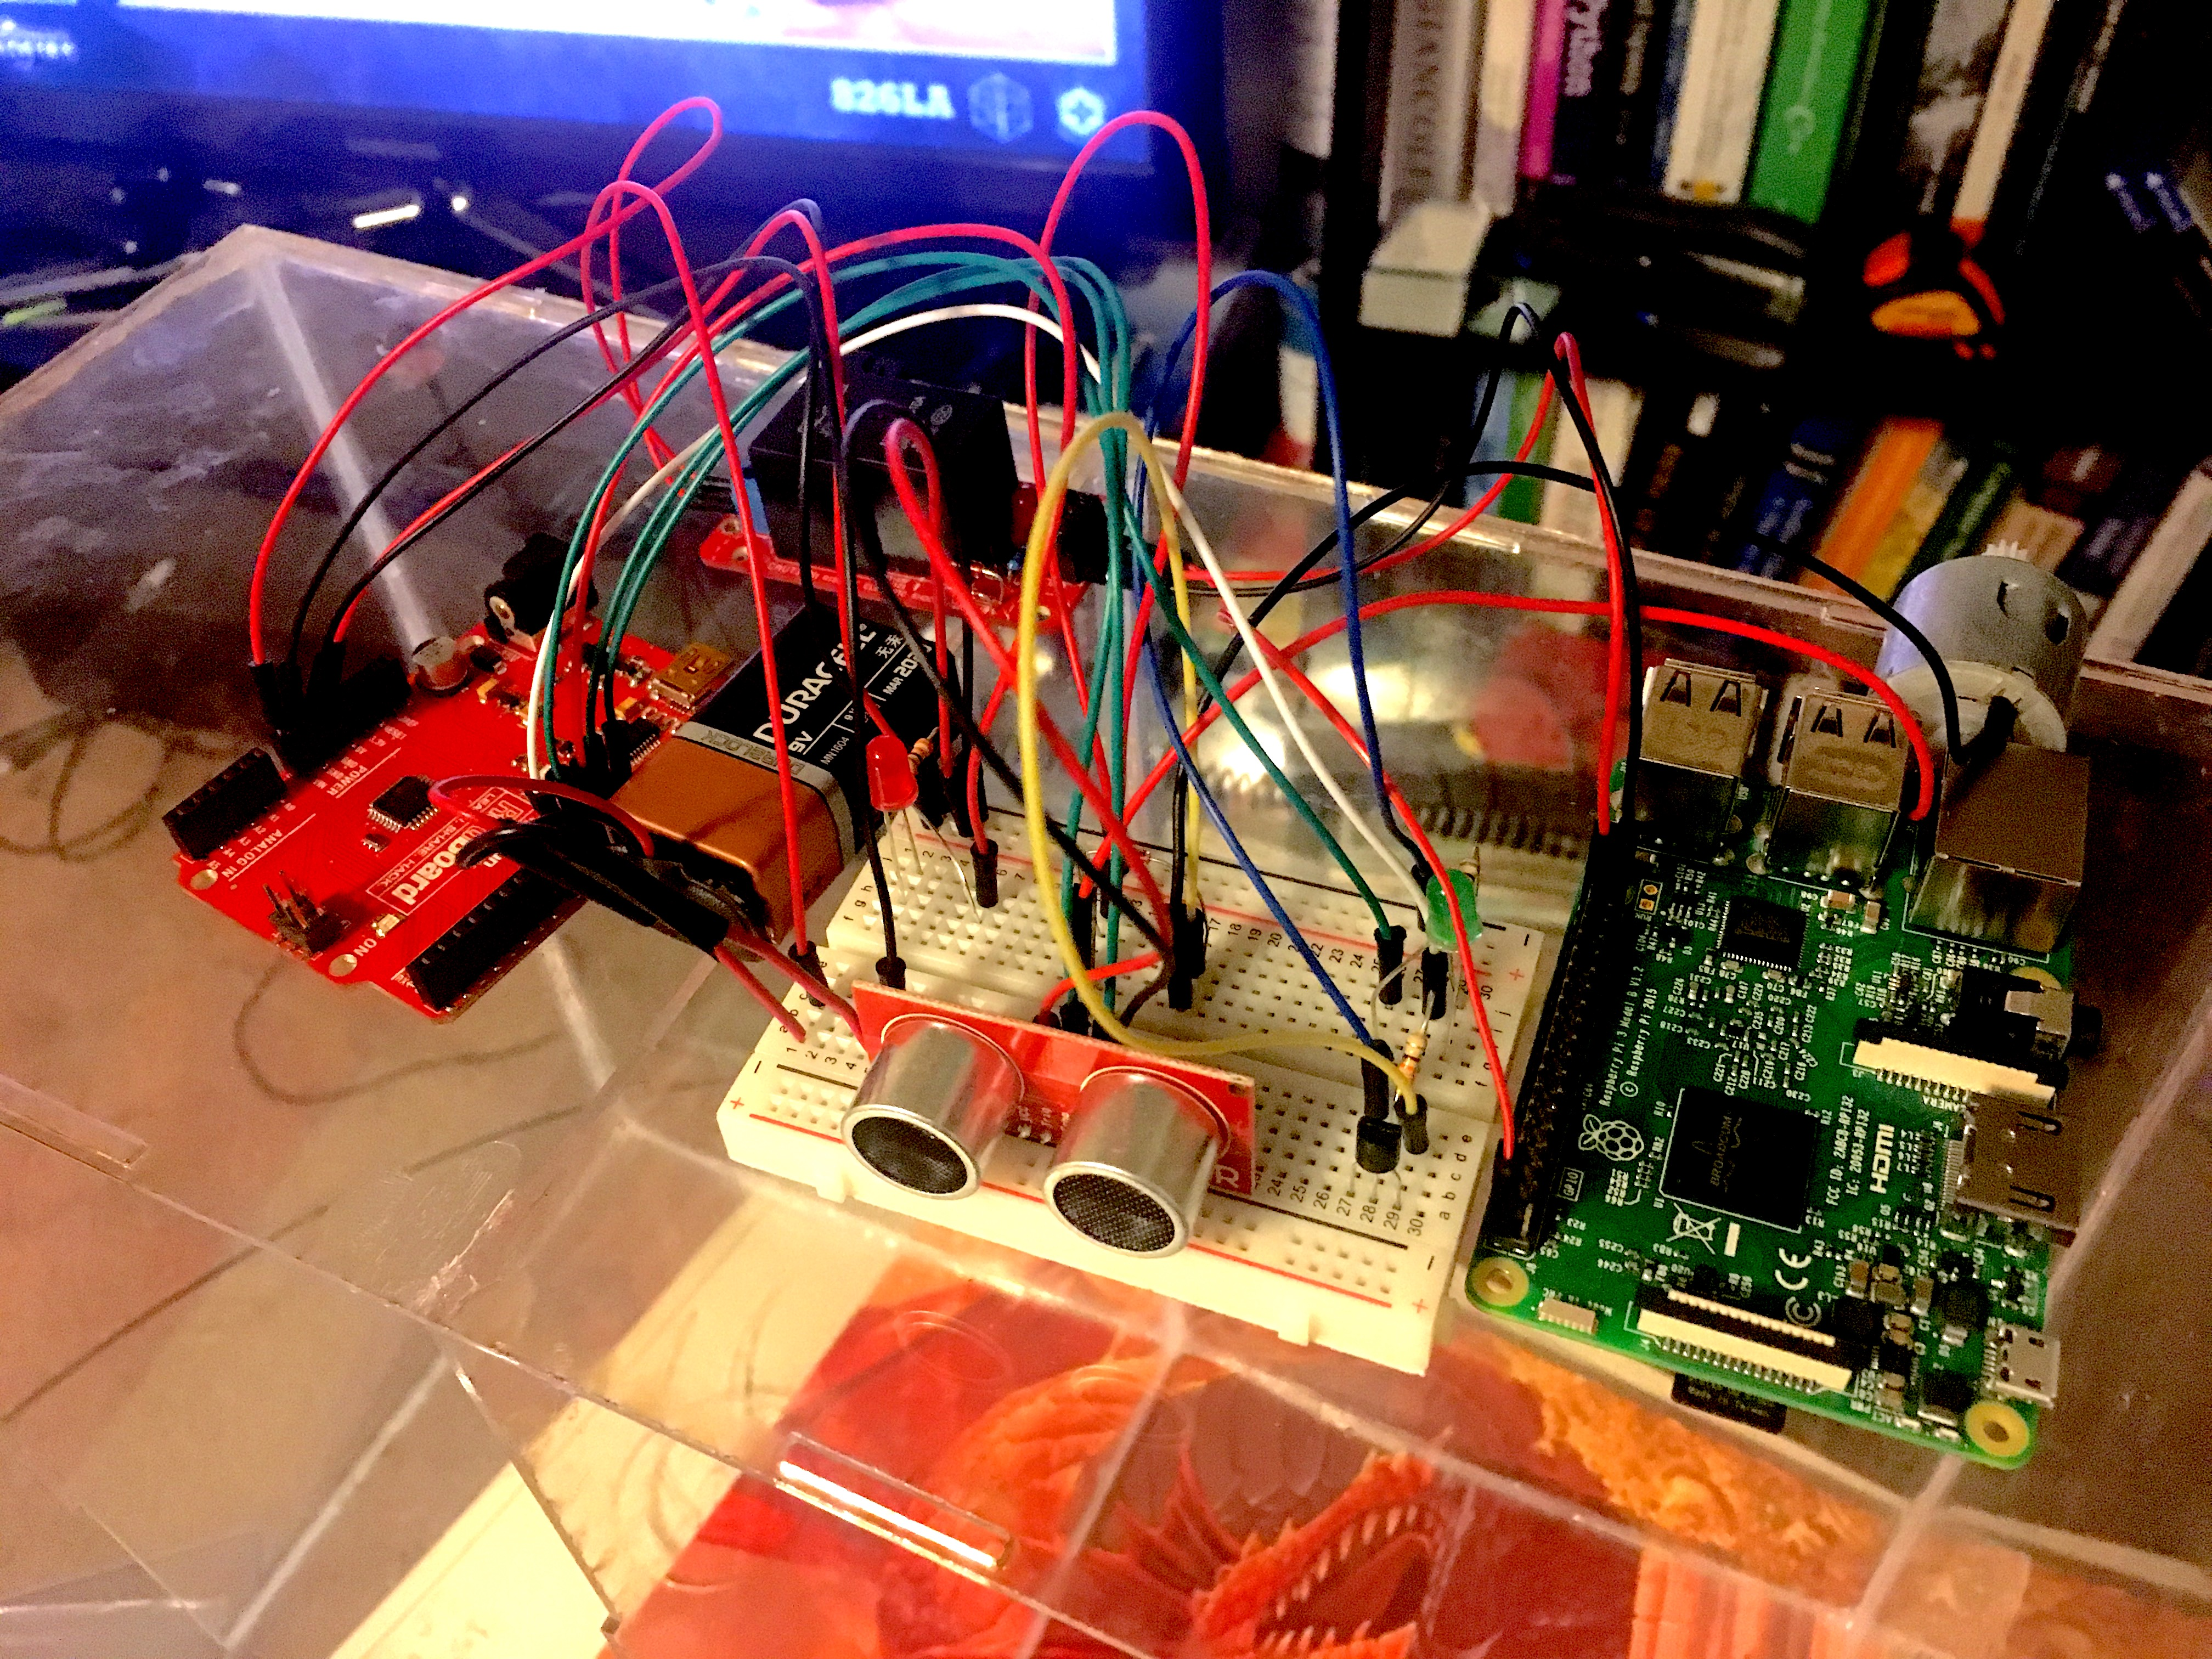
\includegraphics[width=0.75\textwidth]{images/prototype.jpeg}\\ % adds an image from images folder
        \vspace{1cm}     % adds a verticle space of 1cm
        \textbf{MEGN 200}\\    % bold face text
    \end{center}

    \newpage                   % ends page wherever it is and starts what next on new page
    \tableofcontents           % auto generated T.O.C.
    \newpage

    \section{Background}       % New section
        For our project, we decided to create an automatic pet feeder which would use voice control and an app to ensure
        that pets are being fed an adequate amount of food and water. 
        
        There are currently quite a few automatic pet feeders on the market typically ranging from \$30-\$80. Some 
        function by releasing food when the pet places 
        their paw on a certain spot. Others have an option to punch in a feeding schedule and they release food at that 
        time. There is also some voice-controlled options on the market currently, but they tend to be on the higher end 
        of the price range. 
        
        Our goal was to design something similar to what is already on the market but expand it to 
        interface with Amazon Alexa and eventually an app which can set feeding schedules and update the user with the 
        status of their pet's food at any time.

    \section{Problem Statement}

        Keeping up with a household takes a lot of time, effort, and planning. There are so many things that need to be 
        done on a day to day basis that can easily be overlooked in the midst of the modern individual's hectic schedule. 
        According to the 2017-2018 National Pet Owners Survey by the American Pet Products Association, sixty-eight 
        percent of U.S. households are pet owners. Pets require a lot of care including being fed and watered an 
        adequate amount each day in order to stay healthy. Accidentally to feed your pet can cause them to be unhappy 
        and hungry.

        For individuals who are disabled or elderly, adequately caring for pets can be an even greater challenge both 
        physically and mentally. However, pets often provide an irreplaceable comfort and friend to these people. What 
        is needed is an automated pet feeder which can ensure that water bowls are always full and food bowls are being 
        filled to the correct amount each day while being simple enough to manage that it takes little effort or time 
        to control.
        
    \section{Customer Needs}

        To gather information on customer needs, a Google poll was sent out to friends and family. Our team devised two 
        questions to ask to gather data and help define our requirements for the design. The questions are as follows:

        \begin{enumerate}
            \item Of the following products, which would you rank as most useful to you or your home? 
            (Automated lights, Automated watering system, Automated Prt feeder, Automated Fans)
            \item Do you have any cool ideas for a solution to one or many of the above systems?
        \end{enumerate}

        Asking these questions helped to refine the requirements for our design and even a few interesting design ideas 
        that we may not have brainstormed on our own. The results of this poll can be seen in Table \ref{tab:needs}. 
        Based upon these responses, we gathered that an automated pet feeder would be useful and that the market is 
        already full of products like ours. If we were to make a product that clients would desire, we would have to 
        look closely at costs and think outside the box.
        
        \begin{table}[!htb]
            \label{tab:needs}
            \tiny
            \centering
            \begin{tabular}{|C{1cm}|C{1.25cm}|C{14cm}|}
                \hline
                Entry & Question 1 & Question 2 \\
                \hline
                1 & Plants & For plants you could use a pi and some tubing, route water from a large jug into small tubes and use a motor to control drip rate\\\hline
                2 & Plants & Drip type irrigation for potted plants possibly?  \\\hline
                3 & Pet & I've been trying to find affordable LED light panels similar to the aurora Nanoleaf but haven't had any luck.  A lighting system similar to that where could control the colors would be super cool.  \\\hline
                4 & Plant Pets & N/A  \\\hline
                5 & Pet & N/A  \\\hline
                6 & Plant & Plant watering system could recommend watering schedules based on the type of plant you have.  \\\hline
                7 & Light & For the automated plant watering, it seems like I water my plants less when it’s cold and more when it’s hot so if the automated system could adjust to those changes, that would be interesting.  \\\hline
                8 & light & Automated light control that can be used via a smartphone app so you always have a control with you.  \\\hline
                9 & Light & google has many sample projects!  \\\hline
                10 & Plant & Not really. Sorry.   \\\hline
                11 & Pet/Plant & N/A  \\\hline
                12 & All & Implementing daylighting as part of light control (using natural sunlight and having sensors to measure when artificial light is needed)   \\\hline
                13 & Pet & An electronic key fob (like what you use to unlock your car) for my front door sounds super useful.\\\hline
                14 & Pet & Nope!  \\\hline
                15 & Light & Hmmmm... Interfacing any of the three with an app or website could be super useful!  \\\hline
                16 & Plant/Pet & Is there a way to set amount of water as well as time?  \\\hline
                17 & Light/Pet & Sensors?  \\\hline
                18 & All & Machine Learning enabled: Learns your patterns and particular desires  \\\hline
                19 & Pet & Phone application would be great  \\\hline
                20 & Plant/Pet & Homes powered on and off through Bluetooth connection.  \\\hline
                21 & Light & nope  \\\hline
                22 & All & Many timers, automated switches and those little upside down water droplet thingies you put in plants.   \\\hline
                23 & Plant & See Rachio smart phone/web based sprinklers. Great system and control design. Could adapt will to plant watering  \\\hline
                24 & Light & Sensors similar to that of nightlight sensors that automatically adjust lighting as the sun goes down. You could have an app that connects to these to set how bright or dim you want the lights to be at once the kick on into full night time mode.   \\\hline
            \end{tabular}
            \caption{Results of customer survey on Google Poll} 
        \end{table}    

    \section{Design Requirements}
        \begin{table}[!htb]
            \centering
            \begin{tabular}{|c|c|c|c|}\hline
                Metric \# & Metric & Importance (1-5) & Units \\
                \hline
                1 & MSRP & 5 & USD \\
                2 & Size & 4 & sq. ft\\
                3 & Power Consumption & 3 & kWhrs.\\
                4 & Portability & 3 & Yes or No\\
                5 & Feasability for project & 5 & (1 = too long,  5 = too short)\\
                \hline
            \end{tabular}
            \caption{Requirements Breakdown}
        \end{table}

        Based upon the needs that we had seen in the survey and brainstorming what may be a potential metric, we devised 
        five core requirements for our design. Each metric was assigned a unit with which if could be measured and given
        an importance on a scale of 1 to 5 with 5 being necessary and 1 being unnecessary.

    \section{Design Matrix}

        \begin{table}[!htb]
            \label{tab:matrix}
            \centering
            \includegraphics[width=0.75\textwidth]{images/matrix1.png}
            \caption{Problem Solution Design Matrix}
        \end{table}        
        
        We used the design matrix in Table \ref{tab:matrix} to determine what product we should focus our efforts at 
        integrating with our system. The design requirements formed the weights that were applied to each metric. The 
        average weighted scores for each product were then calculated to determine which of the five products we would 
        focus on.

        \begin{table}[!htb]
            \label{tab:matrix2}
            \centering
            \includegraphics[width=0.75\textwidth]{images/matrix2.png}
            \caption{Control System Design Matrix}
        \end{table}

        After determining the product that we would work on, we then applied a secondary matrix seen in Table \ref{tab:matrix2}.
        The purpose of this matrix was to determine which method of interacting with our system we would use. This 
        design decision is more vital than the product used in theory all products should be able to work with this 
        system and the main difference is how the user interfaces with each one. This matrix underwent similar 
        calculations as the previous one, yielding a weighted average score based upon the various metrics.

    \section{Solution Concepts}

        Based on the results of our design matrix, we devised three solutions to create a simple, easy to use, system 
        that could interact with multiple automated systems.  Our three solutions to interfacing with the automated systems 
        were; a phone application, a custom-built touchscreen device, and a voice-controlled system using Amazon Alexa.  
        As this system should work with various different automated systems, we decided to focus 
        on integrating our system with an automated pet feeder.

        \begin{figure}[!htb]
            \centering
            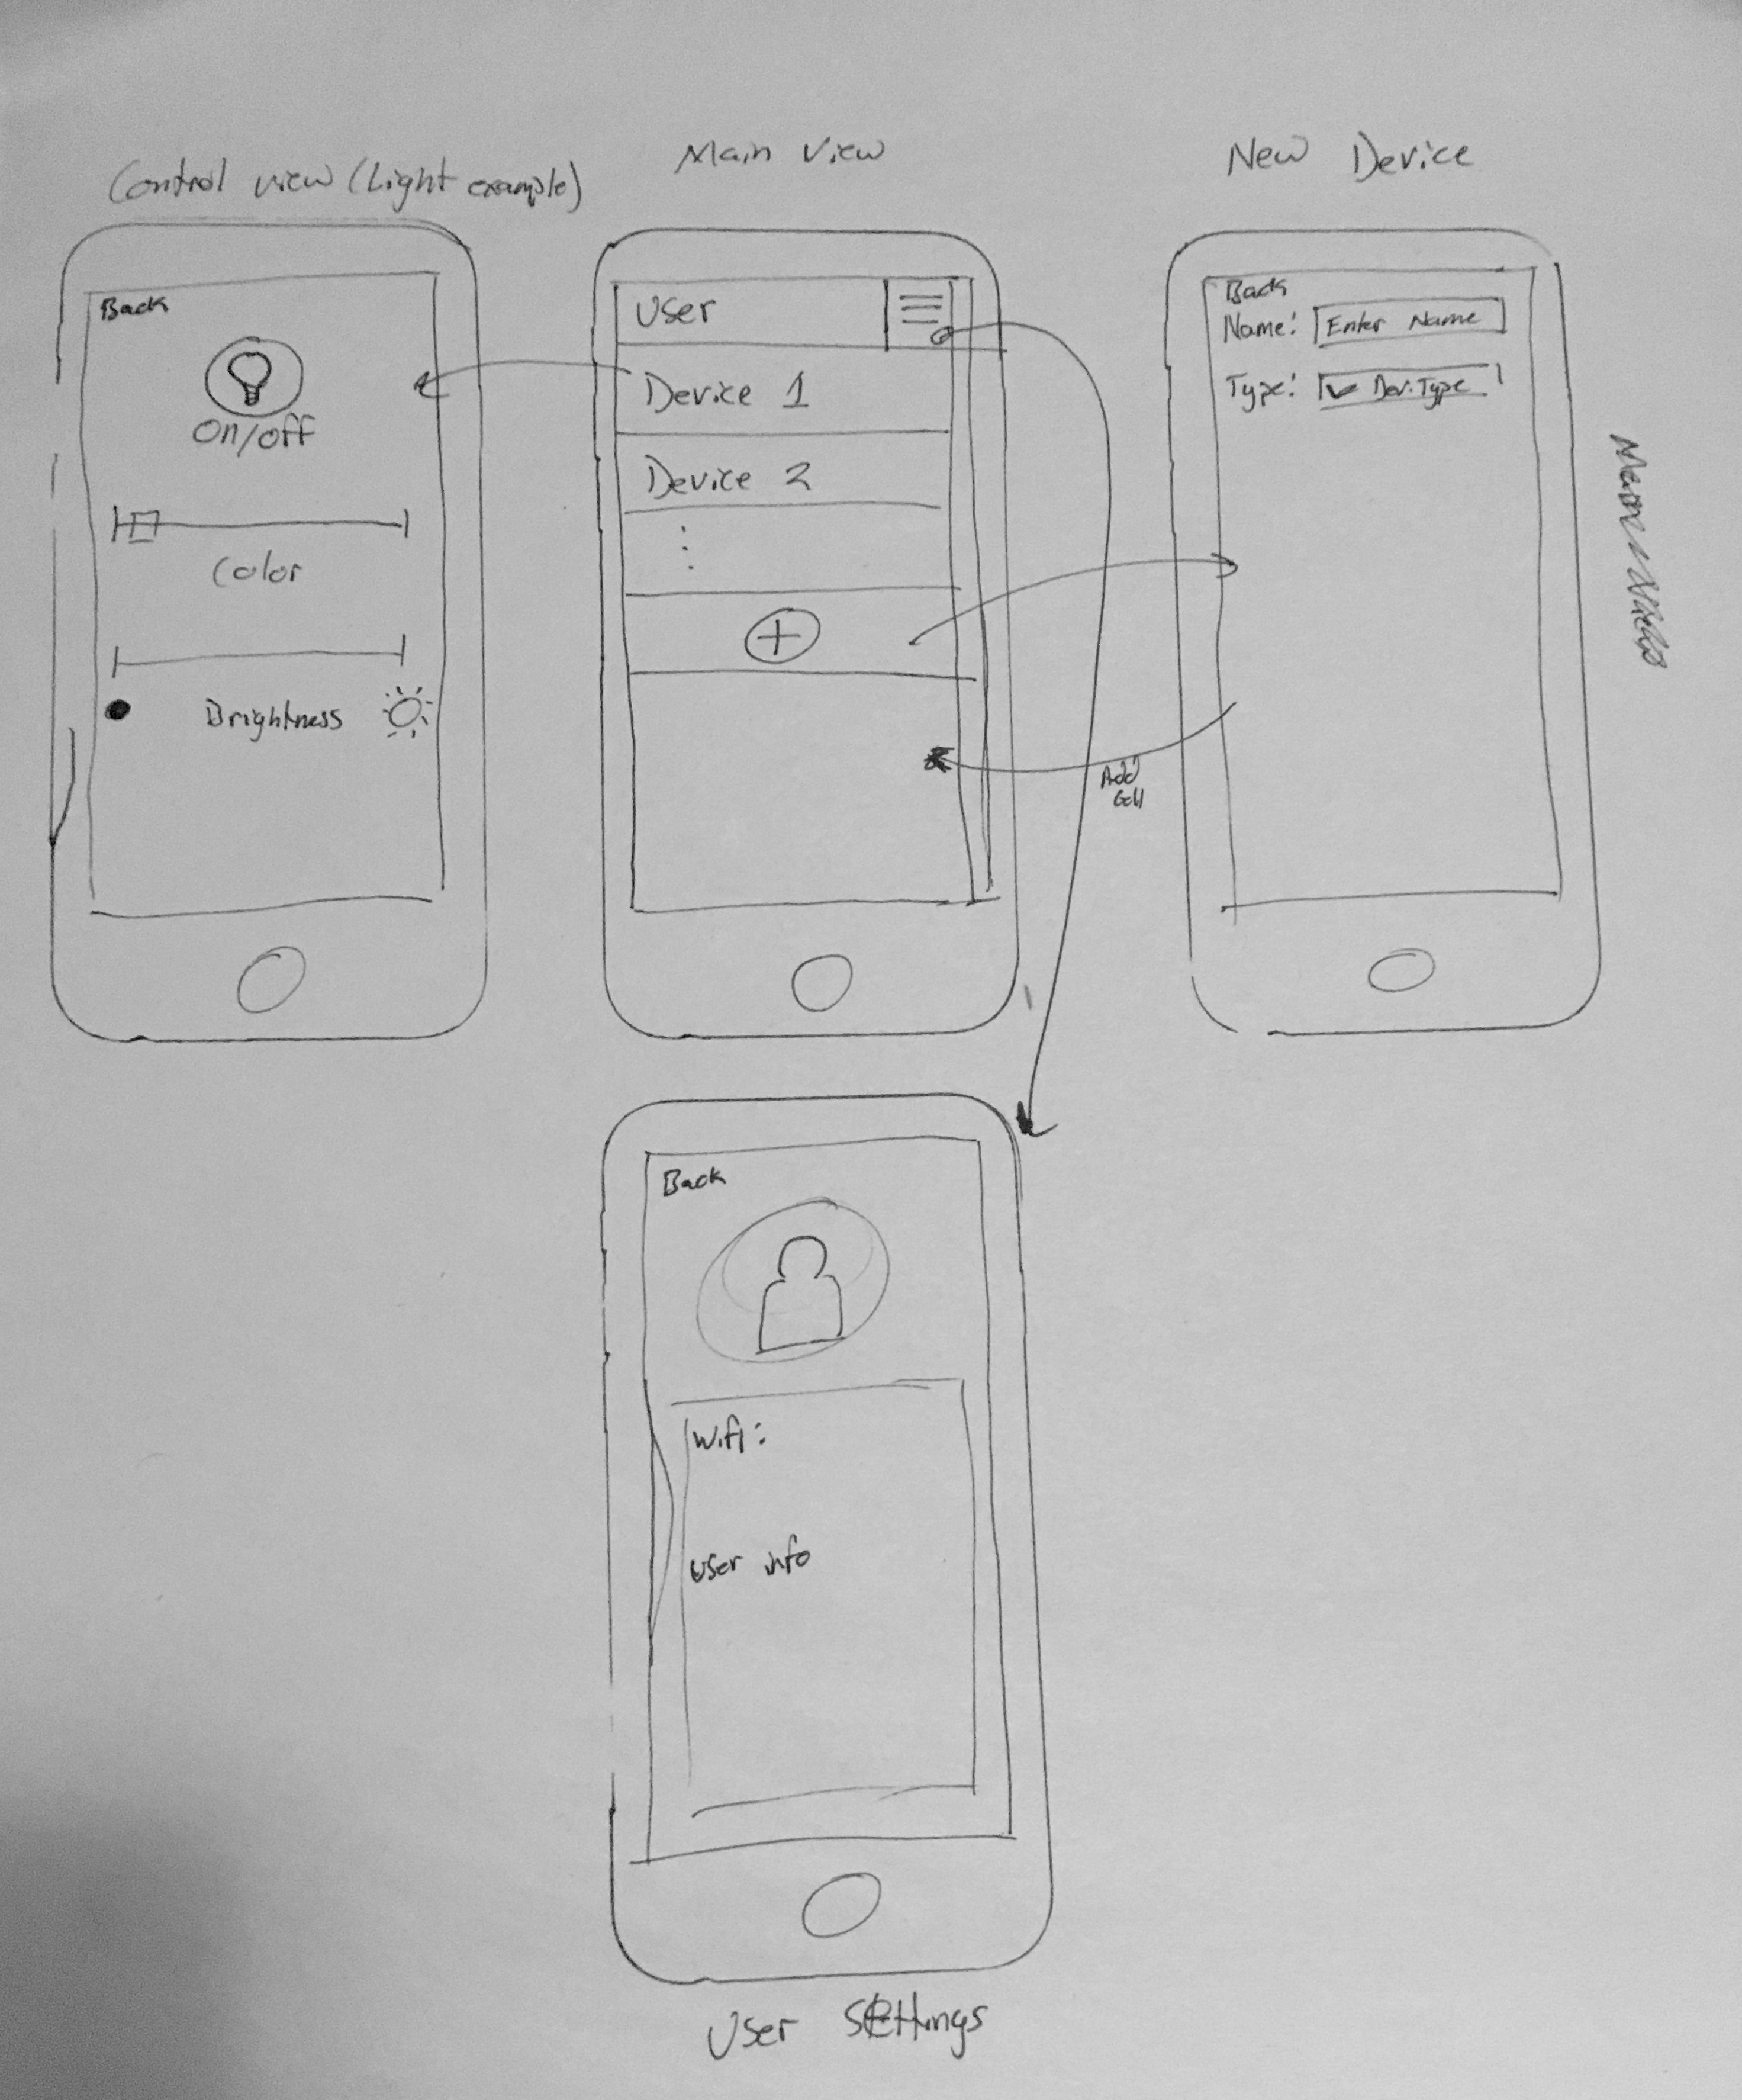
\includegraphics[width=0.5\textwidth]{images/story.jpg}  
            \caption{Application Storyboards}
            \label{fig:story}
        \end{figure}

        The first solution is the least expensive and most intuitive solution in most cases as most everyone that would 
        need this system has a mobile device and are familiar with how to manage and operate applications. The application 
        would have a simple GUI interface and would connect wirelessly to the automated system. Application storyboards 
        were drawn for an iOS device as both members of our team have an iOS phone and can be seen in Figure \ref{fig:story} below.

        The second idea is similar to the first, however, it eliminates the need for the network. A custom touch device 
        that is wired directly to the system would eliminate the need for wireless communication and the need for a 
        mobile device. This idea stemmed from considering how the system could be compromised through a network without 
        proper protection. The storyboards above also provide an adequate example of how this system may look and 
        operate. The downfall of this solution is the setup. In order to connect multiple systems across a home in 
        different locations, so tricky hookups would be required, and it may even have to be installed into a wall if 
        the user wanted an ergonomic look.

        The final model was sparked by considering voice-controlled systems like Iron Man's J.A.R.V.I.S. or the Ship's 
        AI in Star Trek. This solution shines in its' ease of use. Simply walk in the door and ask, "Alexa, what's the 
        status of the house?" to hear a rundown of the various systems that are connected. Additionally, this solution 
        can operate either by purchasing an Alexa supported Amazon product or by connecting a raspberry pi with a 
        microphone to Amazon Web Services(AWS) and utilize the built-in Alexa system to process the users' input, 
        providing this solution more of a DIY option than the other solutions. This design would require a rasPi to set 
        up a server that simulates a WeMo smart home appliance. WeMo is a company that Amazon has partnered with and the 
        devices they develop can sync with Amazon Alexa. The server will simulate the device being a WeMo product and 
        will thus sync without issue. Using a rasPi will also allow for controlled power to the Arduino, turning it on 
        or off when necessary. 

    \section{Final Solution}
 
    \begin{table}[!htb]
            \tiny
            \begin{tabular}{|c|c|c|c|c|c|c|c|}\hline
                Part & Acrylic Sheeting & Hobby Motor & Ultrasonic Sensor-HC-SR04 & Sparkfun Redboard & Raspberry Pi3 & Amazon Echo Dot & Relay Control\\
                Price per Part & \$12.98 & \$1.96 & \$3.94 & \$30.00 & \$20.00 & \$40.00 & \$6.00 \\
                Total &          \$40.00 & \$3.92 & \$3.94 & \$30.00 & \$20.00 & \$40.00 & \$6.00 \\
                Price We Paid  & \$40.00 & \$3.92 & \3.94  & \$0.00  & \$0.00  & \$0.00 & \$0.00 \\
                \hline
            \end{tabular}
            \label{tab:price}
            \caption{Prices and Parts}
        \end{table}

        Based off of our design matrix and the constraints of the small project time span, we decided to design and build
        the Alexa solution. We already had many of the components, thus we ordered what we would need and a few backup sensors
        in the event that some may break during prototyping. See Table \ref{tab:price} for a material pricelist of the 
        signifigant components (excluding wires, diode, and plastic sealant).

        \begin{figure}[!htb]
            \centering
            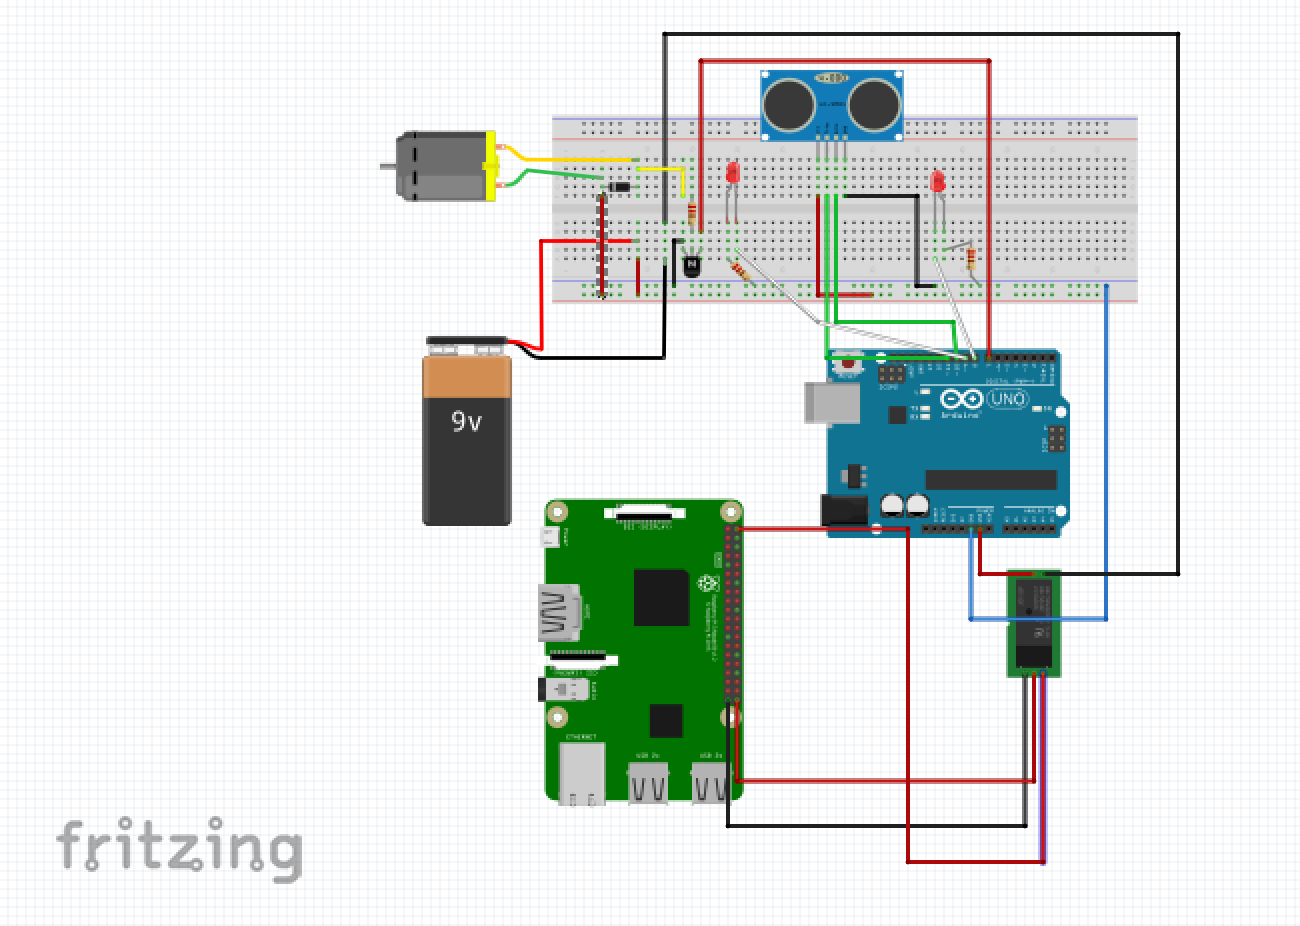
\includegraphics[width=\textwidth]{images/circuit.png}
            \caption{Circuit Diagram}
            \label{fig:circuit}
        \end{figure}

        Once the necessary parts came in, we began working on hooking up the various sensors and slowly added on as we 
        accomplished each step. We worked with an Agile scheme, always having a working system at each stage as to not have 
        a huge system that looks good but doesn't work. After setting up the Alexa services and connecting the raspberry 
        pi to the system, the system appeared as the circuit diagram in Figure \ref{fig:circuit}.

        

        This system works as expected, giving a voice command to the Echo Dot while it is connected to the same network 
        as the RPi sends a signal that is picked up by a script running on the Pi. This is registered as an On/Off switch 
        for the simulated device and a signal is fired through the relay to power the Arduino from a battery for a 
        set number of seconds. During which the code stored on the Arduino would run, checking the depth of the pets' 
        food/water and running the motor if necessary. The purpose of the relay is to prevent the system from continuously 
        running should a sensor go out, as well as to save energy by keeping the Arduino off until needed.
        
        The current prototype of the pet feeder remains incomplete as several internal components needed to be 3D 
        printed after they had been modeled. These components construct the wheel that the motor would rotate to release 
        food and water from the holding cells. After constructing the container, we determined that it may be compromised
        and may not hold water without leaking. 

    \section{Testing}
        The first tests we performed were for testing the readings from the ultrasonic sensor. The primary thing we were
         wondering at this stage was whether or not the sensor would gather similar readings from water as it would from 
         a solid surface. We tested this by running code printing distances that the sensor was receiving in cm, gathering 
         readings from a hand moved in front of it, then holding it over a cup of water. We determined that the sensor did, 
         in fact, receive distance data from the surface of the water. 

        We then moved on to connect two LEDs to determine when something moved within a threshold of the sensor and to 
        switch the lights when this occurred. Once again we tested this with both solid objects and over a cup and even 
        a bowl of water.

        The next tests involved wiring the motor to the system. Using the existing code, we programmed the Arduino to 
        send the motor power from an output pin of the Arduino when outside of the set threshold of 8 cm. (This value 
        would be calibrated based upon distance to the top of a filled dog bowl.) This would start up the motor and cause 
        it to rotate.

        Lastly, we connected the system to the Raspberry Pi and began several small tests to retrieve signals from the 
        Amazon Echo Dot across the network. This was more a trial and error test procedure of printing out statements when 
        signals were received and what they were doing to the system (turning on or off). After several hours of testing 
        and brain scratching, the final tests were passing.

        The next stages of testing would be after the completion of the container, however, this objective was not 
        completed and as such, the remainder of the test could not be completed.
    
    \section{Re-design}
        Our design underwent several changes throughout the course of the construction time. Unfortunately, many on the 
        spot as unforeseen parts were needed to make the system operate the way we desired. In order to power the motor, 
        we discovered that we needed a motor. Additionally, when powering the Arduino from an RPi, a relay switch was 
        needed in order to provide the power up and switching capabilities that were both required to power the Arduino 
        and provide the on-off switching that we desired. Fortunately, Robbie's roommate Caleb Jhones had several of the
        missing components that were needed to complete the project.

        Early on, we had a good idea of what the outside of our container would look like, and what sort of mechanism 
        would funnel and dispense the food, however, we failed to consider that water wouldn't hold itself in the 
        container in the same way that the food would. This issue was never faced, however, this would be a vital next 
        step in the continuation of this prototype. 

    \section{Conclusion}
        Overall, we were satisfied with the progress made on our prototype. We were able to use voice control to start 
        the pet feeder which achieved one of our main goals to make the system hands free. 

        If we were to repeat the process again we would try to obtain better user feedback by asking more specific 
        questions the questions we used to survey potential users were a little vague and so we received vague feedback.

        In the future, as we continue to develop our prototype, we would like to improve the housing and food dispensing 
        systems. We would like to maximize the holding capacity of the reservoirs so that they need to be refilled as 
        infrequently as possible making it easier for individual's who physically have difficulty feeding their pets.

        Additionally, we would like to expand the code so that Alexa can alert the user's when the food or water 
        reservoirs need to be refilled or if there is an issue with the pet feeder which needs to be manually fixed.

        Finally, we would like to develop an app that would let the user control feeding schedules, send notifications 
        to the user's phone when the reservoir needs to be refilled, and let the user check the status of their pets 
        food at any time.

    \newpage

    \section{Code}
        \textbf{testSensors.ino runs on the Arduino to search for depth data and run a motor}
        \lstinputlisting[language=C]{../testSensors.ino} % adds code from a file

    \section{Sources}
    \begin{itemize}
        \item \href{https://github.com/n8henrie/fauxmo}{Alexa to RasPi Hookup}
    \end{itemize}

\end{document}
